\documentclass{article}
\usepackage{graphicx}

\title{Machine, Data and Learning\\
    Assignment 2
}
\author{
    \parbox{0.8\textwidth}{
        Name: Abhinav Reddy Boddu\\
        Roll No: 2021101034\\
    }
}
\date{}
\begin{document}
\maketitle

\section{Task 1: Linear Regression}

\begin{enumerate}
    \item The method $LinearRegression().fit()$ is a function used to train a linear regression model on a given dataset.

    \item  It uses the ordinary least squares (OLS) method to estimate the coefficients of the linear regression model
    \item The method tries to estimate the coefficients of linear model which minimize the sum of the squared residuals between the predicted values and the actual target values.

          \[cost=\mbox{sum of squared residuals} = \sum_{x}(\hat{f}(x) - f(x))^2\]
          \[\mbox{Where x is the input values of data points}\]
          \[\hat{f}(x) \mbox{ is the output predicted by our model for given input x}\]
          \[f(x) \mbox{ is the target values for given input x}\]

    \item It is a supervised learning algorithm used to predict a continuous output variable based on one or more input variables.
    \item The $fit()$ method can handle multiple input variables and can also be extended to include polynomial and interaction terms to model more complex relationships between the input and output variables.
    \item $args$:
        \begin{enumerate}
            \item $X$: input or feature matrix.It is a 2-dimensional array where each row corresponds to a sample or observation, and each column corresponds to a feature or input variable. (independent Variables)
            \item $Y$: This is the other mandatory argument and represents the target or output variable (Dependent Variable)
            \item sample\_weight: The sample weights are used to give more importance to certain observations in the training dataset than others. If not specified, all observations are given equal weight
        \end{enumerate}
\end{enumerate}

\section{Task 2: Gradient Descent}

Gradient descent is an iterative optimization algorithm that can be used to find the coefficients or weights of a machine learning model that minimize a cost function. Where The cost function is a measure of how well the model fits the data and can be defined as the mean squared error between the predicted values and the actual values of the dependent variable.

In the case of a linear regression model with one independent variable and one dependent variable, the goal is to find the slope and intercept of the line that best fits the data.

The basic idea of gradient descent is to update the coefficients iteratively by moving them in the direction of steepest descent of the cost function.


working of gradiant descent method:
\begin{enumerate}
    \item $\textbf{Initialize the coefficients}$: Start with some initial values for the slope (m) and intercept (b) of the linear regression line generally taken as m=0 and b=0.
    \item  $\textbf{Calculate the cost function}$: Calculate the mean squared error between the predicted values of the dependent variable ($y_{pred}$) and the actual values of the dependent variable ($y_{true}$) using the current values of the coefficients.

          \[cost=MSE=\frac{1}{n} \sum(y_{pred} - y_{true})^2\]
    \item  $\textbf{Calculate the gradient}$: Calculate the partial derivatives of the cost function with respect to the slope and intercept.

          \[\frac{d(cost)}{dm} = \frac{d(cost)}{d(y_{pred})} \frac{d(y_{pred})}{dm}\]
          \[\mbox{Since } y_{pred} = mx + b, \frac{d(y_{pred})}{dm} = x\]
          \[\mbox{also } \frac{d(cost)}{d(y_{pred})} = \frac{1}{n}\sum(2(y_{pred}-y_{true}))\]
          \[\Rightarrow \frac{d(cost)}{d(y_{pred})} = \frac{2}{n}\sum((y_{pred}-y_{true}))\]
          \[\Rightarrow gradient_m = \frac{d(cost)}{dm} = \frac{2}{n}\sum(y_{pred} - y_{true}) x\]

          Similarly for b,
          \[\frac{d(cost)}{db} = \frac{d(cost)}{d(y_{pred})} \frac{d(y_{pred})}{db}\]
          \[\mbox{Since } y_{pred} = mx + b, \frac{d(y_{pred})}{db} = 1\]
          \[\mbox{also } \frac{d(cost)}{d(y_{pred})} = \frac{1}{n}\sum(2(y_{pred}-y_{true}))\]
          \[\Rightarrow \frac{d(cost)}{d(y_{pred})} = \frac{2}{n}\sum((y_{pred}-y_{true}))\]
          \[gradient_b = \frac{2}{n}\sum(y_{pred} - y_{true})\]
          \[\mbox{where x is the independent variable.}\]

    \item $\textbf{Update the coefficients}$: Update the values of the slope and intercept by moving them in the direction of steepest descent of the cost function. The size of the update is determined by the learning rate $\alpha$, which is a hyperparameter that controls the step size.

          \[m = m - \alpha*gradient_m\]
          \[b = b - \alpha * gradient_b\]

    \item $\textbf{Repeat steps 2-4 until convergence}$: Repeat steps 2-4 until the

          change in the cost function is below a certain threshold or a maximum number of iterations is reached. Convergence is reached when the coefficients no longer change significantly.

    \item $\textbf{Use the final coefficients}$: Once the algorithm has converged, the final values of the slope and intercept can be used to make predictions on new data.
\end{enumerate}

\section{Task 3.2: Bias \& Variance:}
\begin{center}
    \begin{tabular}{|c|c|c|}
        \hline
        Degree of polynomial & Bias      & Variance    \\
        \hline
        1                    & 0.269416  & 0.00682374   \\
        2                    & 0.0861101 & 0.00130659   \\
        3                    & 0.0335251 & 0.000546639  \\
        4                    & 0.0261134 & 0.000969678  \\
        5                    & 0.0261704 & 0.00148358   \\
        6                    & 0.0269571 & 0.00256623   \\
        7                    & 0.029167  & 0.00645294   \\
        8                    & 0.0338253 & 0.0157929    \\
        9                    & 0.035058  & 0.0240377    \\
        10                   & 0.0296074 & 0.0262106    \\
        11                   & 0.0317448 & 0.0574965    \\
        12                   & 0.0478254 & 0.127828 \\
        13                   & 0.249979  & 4.9005   \\
        14                   & 0.611652  & 6.663    \\
        15                   & 0.845048  & 4.103    \\
        \hline
    \end{tabular}
\end{center}
As the degree of polynomial function increases, the complexity of the model also increases. As a result, both the bias and variance of the model may change.

\pagebreak
\subsection{Simpler model(Polynomials of lower degree)}

A less complex model generally does not recognize the pattern in the data i.e it underfits the data, therby predicted output of the model and the actual output (i.e Bias) differ greately.

But then recognizing less pattern means the model can fit to any general data, Thereby very low variance

Thereby a less complex model causes more bias and less Variance compared to relatively more complex model

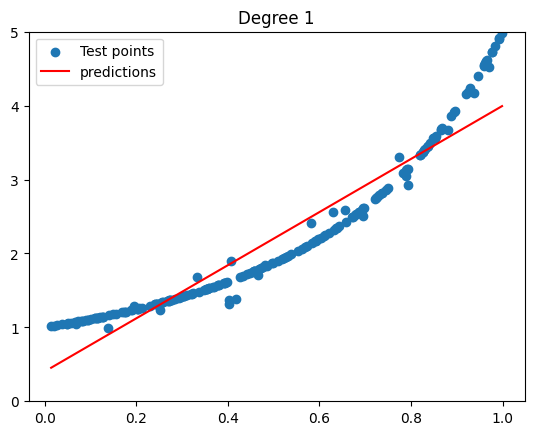
\includegraphics{model-00.png}


\pagebreak
\subsection{Complex models(Polynomials of higher degree)}

A complex model generally does recognizes more pattern in the data than required i.e it overfits the data, therby predicted output of the model and the actual output (i.e Bias) differ by very small values.

But then recognizing more pattern means the model can't fit to any general data, Thereby higher variance from test case to test case

Thereby a more complex model causes less bias and high Variance compared to relatively simple models

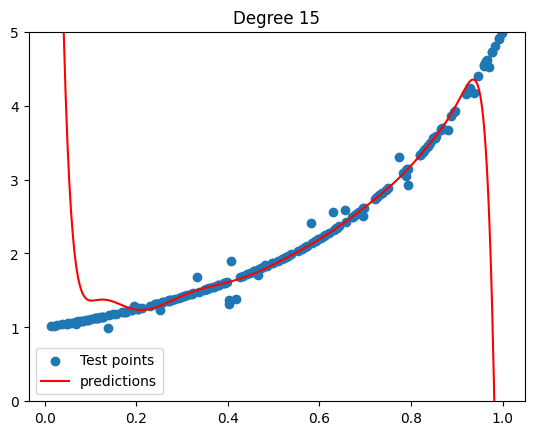
\includegraphics{model-150.png}

\section{Task 4: Irreducible error}
\begin{center}

    \begin{tabular}{|c|c|}
        \hline
        Degree of polynomial & Irreducible error  \\
        \hline
        1         & -5.19116$\times 10^{-18}$   \\
        2         & -1.16498$\times 10^{-18}$   \\
        3         & -1.95536$\times 10^{-18}$   \\
        4         & -4.57127$\times 10^{-19}$   \\
        5         & -1.36975$\times 10^{-18}$   \\
        6         &  2.46548$\times 10^{-18}$   \\
        7         & -3.32931$\times 10^{-18}$   \\
        8         &  1.65883$\times 10^{-19}$   \\
        9         &  5.00305$\times 10^{-18}$   \\
       10         &  2.91713$\times 10^{-17}$   \\
       11         & -1.11784$\times 10^{-17}$   \\
       12         &  8.90867$\times 10^{-17}$   \\
       13         &  6.04636$\times 10^{-16}$   \\
       14         & -5.87047$\times 10^{-15}$   \\
       15         & -1.39834$\times 10^{-14}$   \\
 
        \hline
    \end{tabular}

\end{center}

The irreducible error is the error that cannot be reduced by any model, regardless of its complexity. It is a result of the noise inherent in the data or any other unpredictable factors that affect the dependent variable. As such, the value of the irreducible error should not change as we vary our class function, as it is not dependent on the model itself.

It is called irreducible because it cannot be eliminated by any improvements in the model

\section{Task 5: $\textbf{Bias}^2$ , Variance tradeoff}
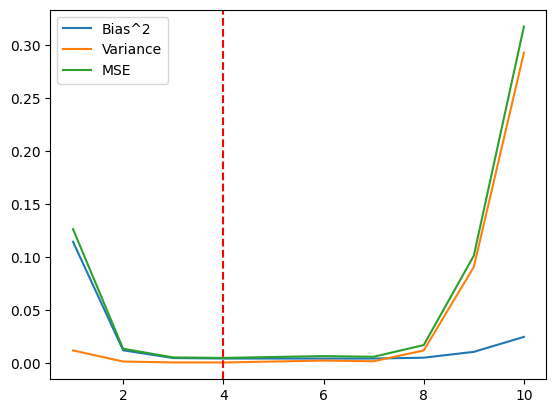
\includegraphics{output-1.png}

\subsection*{Key observations of $\mbox{Bias}^2$-Variance Graphs:}
\begin{enumerate}
    \item $\textbf{Underfitting}$: We can observe that the polynomial models with degrees 1-2 have high bias ($underfitting$) because they are too simple to capture the complexity of the data. These models are not able to fit the training data well and have high MSE (total error). Therefore, they are not suitable for the given data.

    \item $\textbf{Overfitting}$: We can observe that the polynomial models with degrees $>$ 8 have high variance ($overfitting$) because they are too complex and capture the noise in the training data. These models have low bias but high MSE (total error) because they fit the training data too well and do not generalize well to new, unseen data. Therefore, they are not suitable for the given data.
    
    \item $\textbf{Good fit}$: We can observe that the polynomial models with degrees 3-7 have the best balance between bias and variance and achieve the lowest MSE (total error). These models are able to capture the complexity of the data without overfitting, and they generalize well to new, unseen data. Therefore, they are good fit models for the given data.
    
    \item $\textbf{Type of data}$: The $\mbox{Bias}^2$-Variance plot suggests that the data has a non-linear relationship between the input features and the target variable, as indicated by the U-shaped curve. It also suggests that there may be some noise in the data, as indicated by the high MSE (total error) across all polynomial degrees. Therefore, it may be necessary to preprocess the data to reduce noise or transform it to a more appropriate format before fitting a polynomial regression model.
\end{enumerate}
\section{Bonus:}
Given: \[Q=CV_0e^{-\frac{t}{RC}}\]

We can clearly see it is not linear.

On applying $\ln()$
\[\ln Q = \ln(CV_0e^{-\frac{t}{RC}}) = \ln(CV_0) - \frac{t}{RC}\]

i.e $\ln Q$ and $t$ are linearly related,

We can find $\ln Q$ values from given $Q$, then find the coefficients and intercepts of $\ln Q = mt + c$,

$m=-\frac{1}{RC}$ and $c= \ln(CV_0)$

\[\Rightarrow CV_0 = e^c\]
\[\Rightarrow C = \frac{e^c}{V_0}\]

Also,
\[RC=-\frac{1}{m}\]
\[\Rightarrow R=-\frac{1}{Cm}=-\frac{1}{\frac{e^c}{V_0}m}=-\frac{V_0}{e^cm}\]

\framebox[0.9\textwidth]{
    \parbox{0.7\textwidth}{
        \begin{center}
            $\textbf{Obtained Values}$
        \end{center}
        $R\approx 10^5$

        $C\approx 5\times10^{-5}$
    }
}
\end{document}